\documentclass[UTF8,9pt]{ctexart}
\usepackage{../../template/homeworkTEMP/hw}
\setcounter{secnumdepth}{0}
    \title{理论力学 hw2}  
\begin{document} 
\maketitle 
\section{Q1}
    记静止系中坐标为$r$, 运动系中为$r'$, 设引力为$G$, 则:
    $$\begin{array}{rl}
        a=&\dt{\,'\bm{r}} \\   
         =&(\dt{ \,' }+\bm{\omega}\times)^2\bm{r}\\
         =&\dt[2]{\,'\bm{r}}+2 \bm{\omega} \times \dt{\,'\bm{r}}+\bm{\omega}\times(\bm{\omega}\times \bm{r})\\
         =&\bm{a}'+2\bm{\omega}\times \bm{v}'+(\bm{\omega}\cdot \bm{r})\bm{\omega}-\bm{\omega}^2\bm{r}=\bm{F}_N/m-\bm{g}\\  
         \Rightarrow \bm{a}'=&\bm{F}_N/m-\bm{G}/m-2\bm{\omega}\times \bm{v}'+\bm{\omega}^2\bm{r}\cos\lambda 
    \end{array}$$
    记$m\bm{g}=\bm{G}-m\bm{\omega}^2\bm{r}\cos\lambda$为重力。垂直运动方向为$z$轴,水平方向为$x,y$方向,且初速度$v_0$沿$x$方向, \\
    由于桌面约束,$a'_z=0$,\\
    由于$mg$和$F_N$垂直于$z$轴,$a_x=a_y=0$,\\则有:
    $$\bm{a}'=\bm{F}_N/m-\bm{g}-2\bm{\omega}\times \bm{v}'$$
    $$\bm{\omega}\times \bm{v}'=\omega\left|\begin{matrix}
        \bm{i} & \bm{j} & \bm{k}\\
        -\cos\lambda & 0 & \sin\lambda\\
        \dot{x} & \dot{y} & \dot{z}
    \end{matrix}\right|$$ 
    $$\Rightarrow \left\{\begin{array}{rll}
        m\ddot{x}=&2m\omega\dot{y}\sin\lambda\\
        m\ddot{y}=&-2m\omega \dot{x}\sin\lambda\\
        m\ddot{z}=&F_N-mg+2m\omega\dot{y}\cos\lambda&=0\\
    \end{array}\right.$$
    求解上述方程,代入初值$\dot{x}(0)=v_0$,容易看出:
    $$\left\{\begin{array}{rll}
        \dot{x}=&v_0\cos (2\omega\sin\lambda t)\\
        \dot{y}=&-v_0\sin (2\omega\sin\lambda t)\\
    \end{array}\right.$$
    $$\left\{\begin{array}{rll}
        x=&\f{v_0}{2\omega\sin\lambda}\sin (2\omega\sin\lambda t)\\
        y=&\f{v_0}{2\omega\sin\lambda}(\cos (2\omega\sin\lambda t)-1)\\
    \end{array}\right.$$
    合并上式,有:
    $$x^2+\left(y+\f{v_0}{2\omega\sin\lambda}\right)^2=\left(\f{v_0}{2\omega\sin\lambda}\right)^2$$
    这是一个圆方程,说明其轨迹是一个圆周,且半径$r=\f{v_0}{2\omega\sin\lambda}$.\\
    将$\dot{y}$代入$F_N$表达式,桌面支持力为:
    $$F_N=mg+2m\omega v_0 \cos\lambda\sin (2\omega\sin\lambda t)$$
    由于桌面与物体在$z$方向无相对加速度,支持力与压力相等:
    $$F_0=F_N=mg+2m\omega v_0 \cos\lambda\sin (2\omega\sin\lambda t)$$
\section{Q2}
    \subsection{}
        \begin{center}
            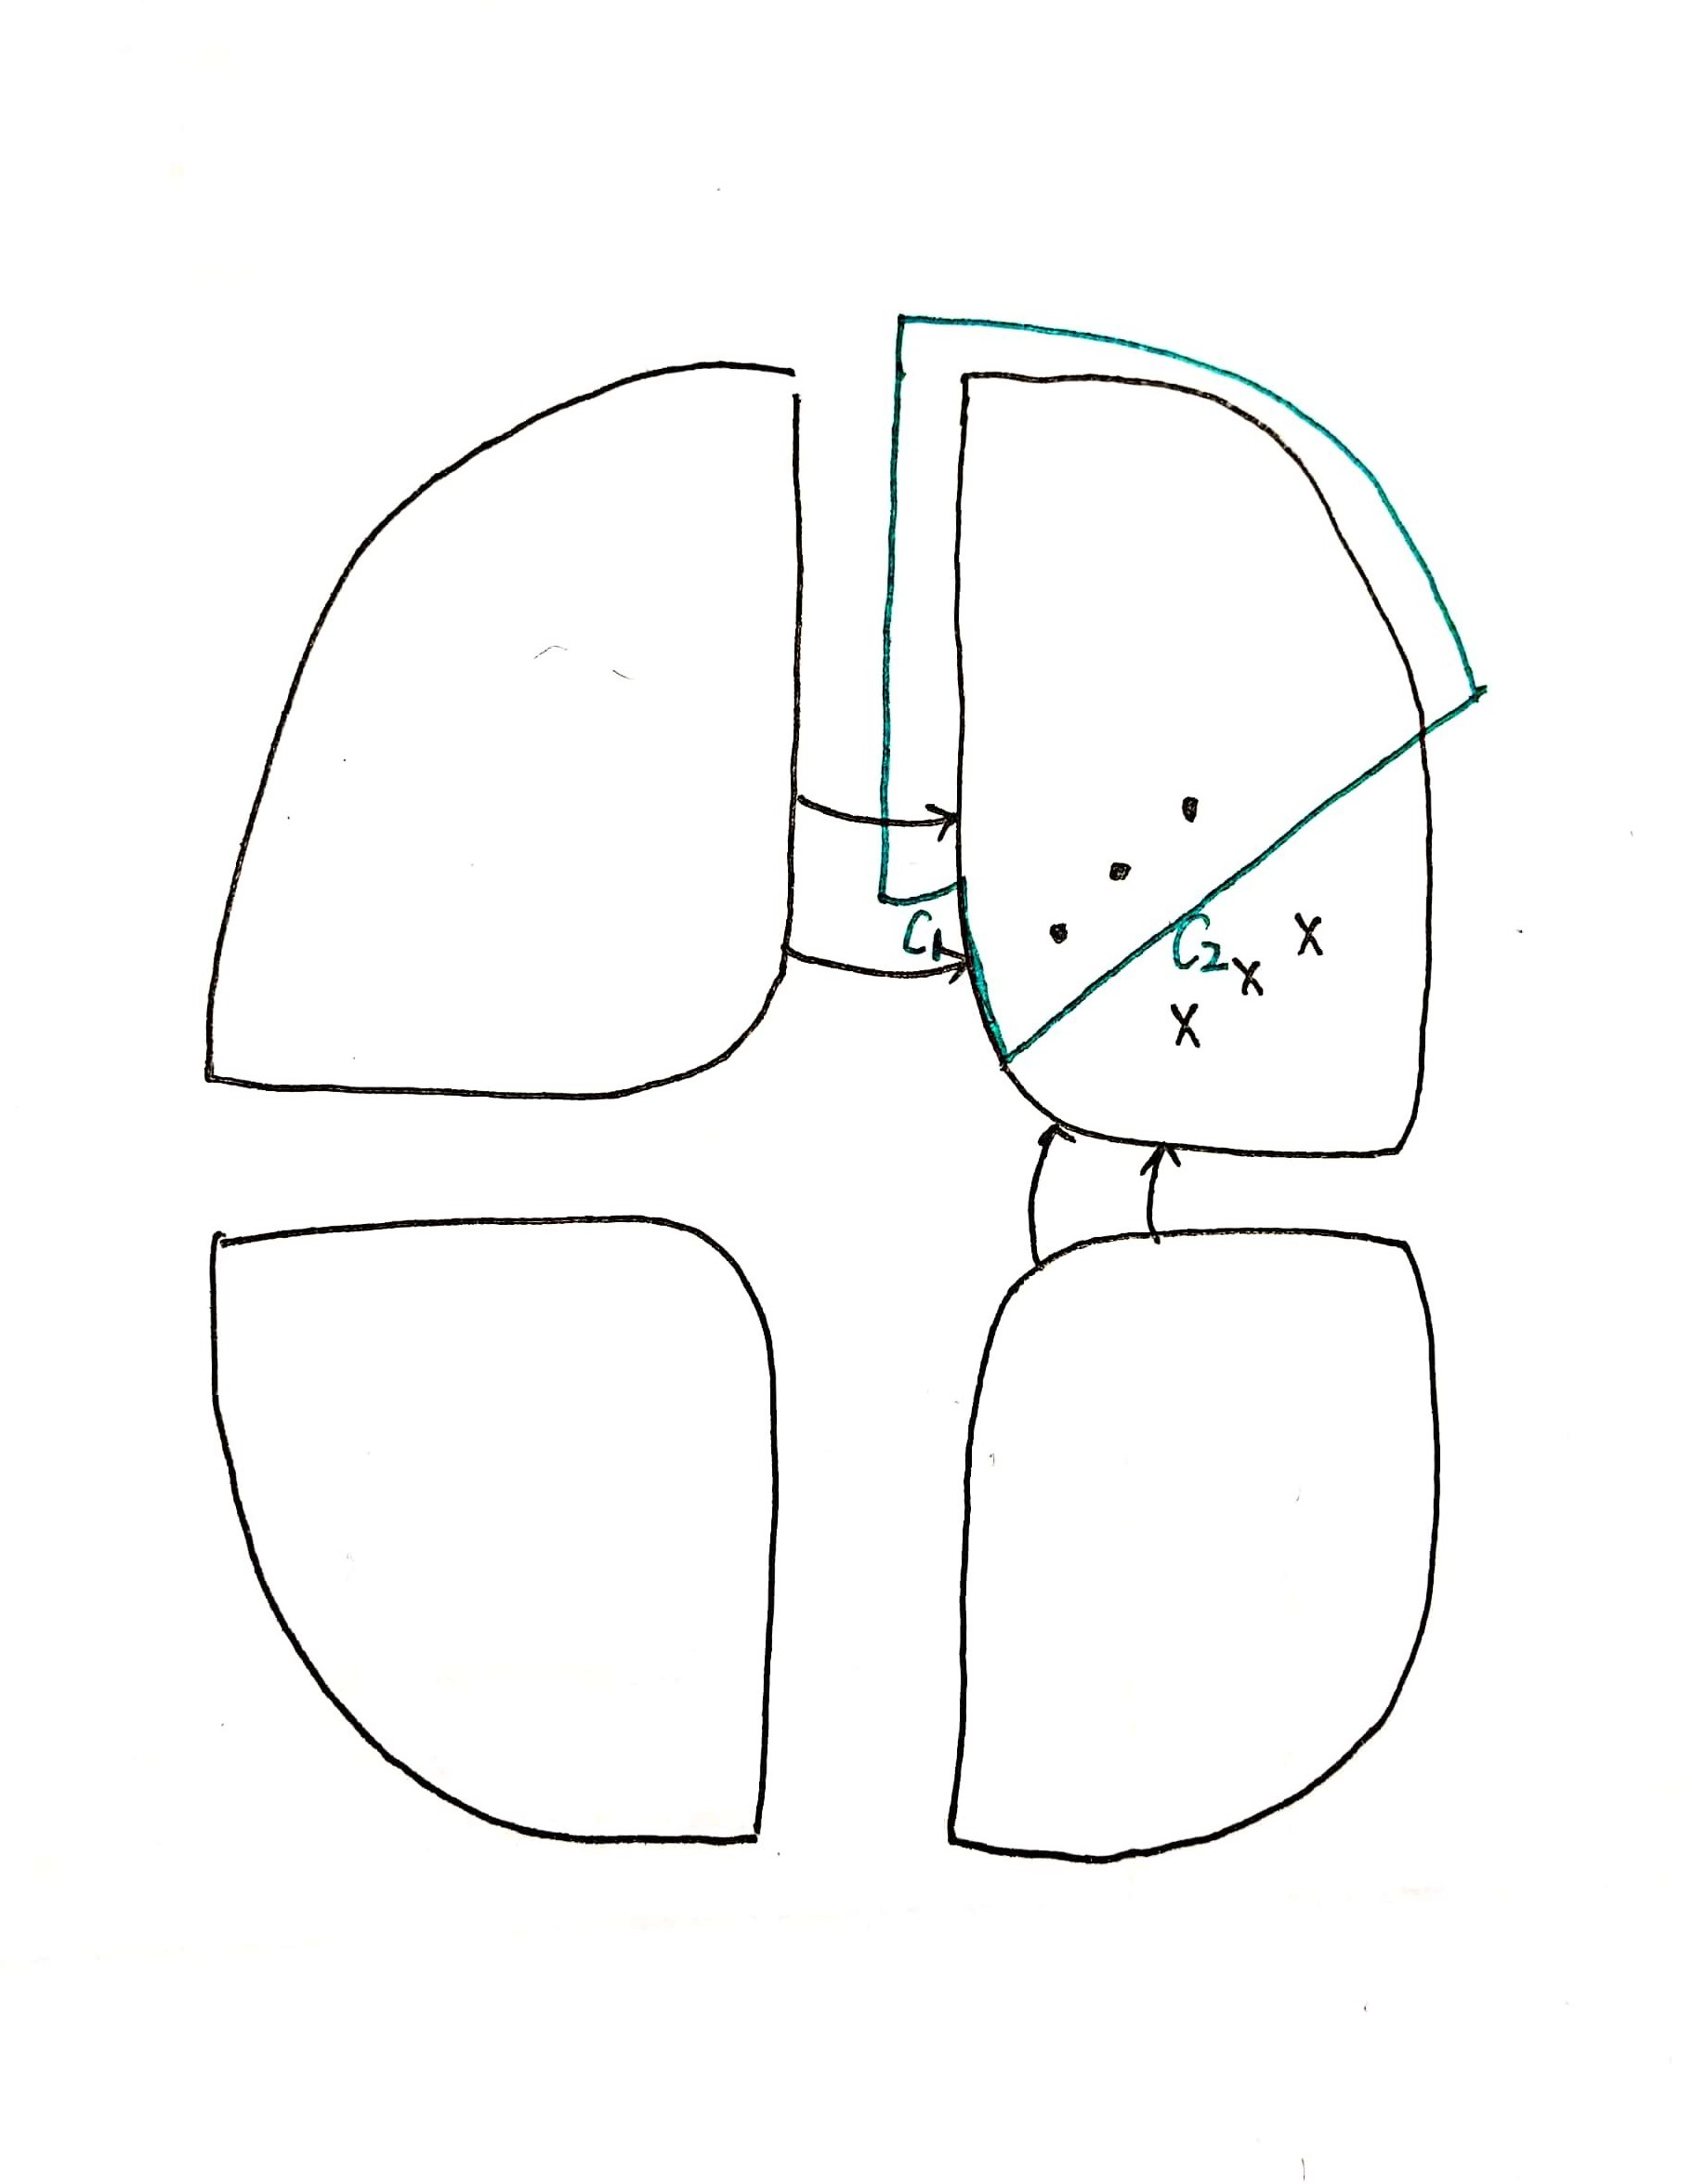
\includegraphics[scale=0.6]{1.jpg}\\ 
        \end{center}
        如上图所示,$A,B$两点有速度$u,v$,作速度垂线,交于$D$,$D$即为转动瞬心.\\
        以$D$为基点. 设$\angle ABO=k$,$AM=a, BM=b$.
        显然:
        $$\begin{array}{rl}
            x=&b\sin k\\
            y=&a\cos k\\
            \omega=&\frac{u}{(a+b)\sin k}\\
            \Rightarrow\qquad
            \dot{x}=&b\cos k \omega\\
            =&\frac{b u\cot k}{a+b}\\
            \dot{y}=&-a\sin k \omega\\
            =&\frac{-au}{a+b}\\
            \Rightarrow\qquad
            \ddot{x}=&\frac{-bu^2}{(a+b)^2\sin^3k}\\
            \ddot{y}=&0\\
            a=&\sqrt{\ddot{x}^2+\ddot{y}^2}\\
            =&\frac{-bu^2}{(a+b)^2\sin^3k}
        \end{array}$$  
        
        
    \subsection{}
        如上一问分析,瞬心S即为图中D点。
\section{Q3}
    \subsection{}
        $$\begin{array}{rl}
            I_x=I_y=&\rho\int_{-r}^rdz\int_0^rrdr\int_0^{2\pi}(r^2\cos^2\theta+z^2)d\theta\\
            =&\frac{7}{6}\pi r^5\rho\\
            And \quad \rho=&m/V=\frac{m}{2\pi r^3}\\
            \Rightarrow I_x=I_y=&\frac{7mr^2}{12}\\
            \\
            I_z=&\rho\int_{-r}^rdz\int_0^rrdr\int_0^{2\pi}r^2d\theta\\
            =&\pi r^5\rho\\
            And \quad \rho=&m/V=\frac{m}{2\pi r^3}\\
            \Rightarrow I_z=&\frac{mr^2}{2}\\
            \Rightarrow \vec{\vec{I}}=&\begin{bmatrix}
                \frac{7mr^2}{12} & 0 & 0\\
                0 & \frac{7mr^2}{12} & 0\\
                0 & 0 & \frac{mr^2}{2}
            \end{bmatrix}
            \\
            I=&I_xcos^2 90+I_y\cos^2 30+I_z\sin^2 30+m(\sqrt{2}r\cdot \sin75)^2\\
            =&(\frac{9}{16}+\frac{\sqrt{3}}{2})mr^2
        \end{array}$$  
    \subsection{}
        $$\begin{array}{rl}
                \vec{J}=&I\vec{\omega}, \quad \vec{\omega}=(0 \  \frac{\sqrt{3}\omega}{2} \  \frac{\omega}{2})\\
                \vec{J}=&(\frac{9}{16}+\frac{\sqrt{3}}{2})mr^2 \cdot \vec{\omega}\\
                \vec{J}=&\left(0,\ \frac{3}{4}+\frac{9\sqrt{3}}{32},\  \frac{\sqrt{3}}{4}+\frac{9}{32}\right)m\omega r^2

        \end{array}$$  
\section{Q4}
    \subsection{}
        \begin{center}
            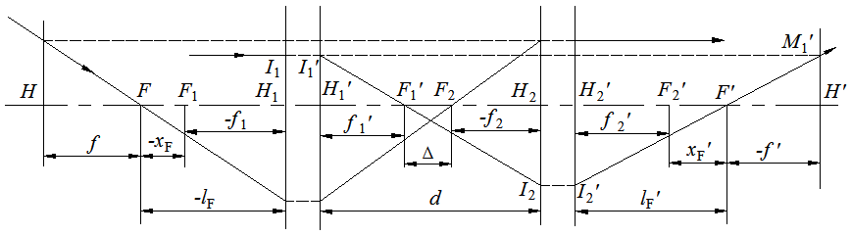
\includegraphics[scale=0.4]{2.png}\\
        \end{center}
            如上图所示,以A为基点,由能量守恒可知:
            $$\begin{array}{rlr}
                \frac{I\omega^2}=&\frac{mgl}{2}(\sin\varphi_0-\sin\varphi)\\
                \frac{1}{6}ml^2\omega^2=&\frac{mgl}{2}(\sin\varphi_0-\sin\varphi)\\
                \omega^2=&\frac{3g}{l}(\sin\varphi_0-\sin\varphi)\\
                \Rightarrow \omega=&\sqrt{\frac{3g}{l}(\sin\varphi_0-\sin\varphi)} & \qquad(1)\\
                \text{两边求导:}\\
                2\omega \alpha=&-\frac{3g}{l}\cos\varphi \dot{\varphi}\\
                \Rightarrow \alpha=&\frac{3g}{2l}\cos\varphi & (2)\\
            \end{array}$$ 
    \subsection{}
    $$\begin{array}{rl}
        F_A=&mg+m\ddot{y_c}\\
        F_B=&m\ddot{x_c}\\
        x_c=&\frac{l}{2}\cos\varphi\\
        \ddot{x_c}=&-\frac{l}{2}(\cos\varphi \dot{\varphi}^2+\sin\varphi\ddot{\varphi})\\
        y_c=&\frac{l}{2}\sin\varphi\\
        \ddot{y_c}=&\frac{l}{2}(-\sin\varphi \dot{\varphi}^2+\cos\varphi\ddot{\varphi})\\
        \text{综上,}\qquad\\
        F_A=&mg-\frac{l}{2}m\sin\varphi\ddot{\varphi}\\
        =&(1+\frac{3}{4}\sin\varphi\cos\varphi)mg\\
        F_B=&-\frac{l}{2}m\sin\varphi\ddot{\varphi}\\
        =&\frac{3}{4}\sin\varphi\cos\varphi mg\\
        

    \end{array}$$ 
    \subsection{}
    $$\begin{array}{rlr}
        x_c=&\frac{l}{2}\cos\varphi\\
        \text{当}\quad \ddot{x}_c=&-\frac{l}{2}(\cos\varphi \dot{\varphi}+\sin\varphi\ddot{\varphi})=0\\
        \cos\varphi\omega^2= & \sin\varphi\alpha & (3) \\
        \text{综合(1)(2)(3),}\\
        2\sin\varphi_0=&3\sin\varphi\\
        \Rightarrow \varphi=&\arcsin(\frac{2}{3}\sin\varphi_0)

    \end{array}$$ 
\section{Q5} 
    垂直于槽,在纸面内n方向:
    $$F_n=mg\sin\alpha - \frac{mv_y^2}{s\ \sin\alpha}\cos\alpha$$
    沿着槽t方向:

    $$\begin{array}{rl}
        v_t=&\int a_t dt\\
        ma_t=&mg \cos\alpha + \frac{mv_y^2}{s}
    \end{array}$$  
    垂直于槽和纸面y方向: 
    $$\begin{array}{rl}  
        v_y=&\omega\,s\,\sin\alpha\\
        F_y=&\dt{mv_y}\\
        =&m\dt{}(\omega\,s)\sin\alpha\\
            =&m\omega v_t \sin\alpha\\
        \ddot{s}=&a_t\\
        \ddot{s}=&g\cos\alpha + \omega^2\sin^2\alpha s\\
        
        s=& \frac{g \cos\alpha e^{- t\omega \sin\alpha} \left(e^{t\omega \sin\alpha}-1\right)^2}{2\omega^2 \sin^2\alpha}\\
        v_t=&\frac{g \cot \alpha e^{-t \omega \sin\alpha} \left(e^{2 t \omega \sin\alpha}-1\right)}{2 \omega}
    \end{array}$$
    则有:
    $$\begin{array}{rl}
        F_n=&mg\sin\alpha-m\omega^2s\,\sin\alpha \cos\alpha\\
        F_y=&m\omega \sin\alpha v_t\\
            =&\ff{2}m g \cos\alpha e^{-t \omega \sin\alpha} \left(e^{2 t \omega \sin\alpha}-1\right)\\
        F_N=&\sqrt{F_n^2+F_y^2}\\
        =&\sqrt{\left(mg\sin\alpha - m\omega^2s\,\sin\alpha \cos\alpha\right)^2+\left(\ff{2}m g \cos\alpha e^{-t \omega \sin\alpha} \left(e^{2 t \omega \sin\alpha}-1\right)\right)^2}
    \end{array}$$
\end{document}
    
    